%!TEX root = ./template-skripsi.tex
%-------------------------------------------------------------------------------
%                            BAB V
%               		HASIL DAN PEMBAHASAN
%-------------------------------------------------------------------------------

\chapter{IMPLEMENTASI DAN PENGUJIAN}
	\section{\emph{Coding} (Implementasi Sistem)}
	Berdasarkan hasil analisis dan perancangan yang telah dilakukan sebelumnya, peneliti berlanjut melakukan tahap implementasi.
	    \subsection{Implementasi Basis Data (\emph{Database})}
	    Implementasi basis data (\emph{database}) ini merupakan hasil pembuatan tabel pada \emph{database} berdasarkan hasil perancangan tabel sebelumnya. Peneliti menggunakan \emph{phpMyAdmin} untuk mengelola \emph{database MySQL}. Hasil implementasi basis data adalah sebagai berikut:
	    \begin{enumerate}
	        \itemsep0em
	        \item Tabel Master Bidang (\texttt{master\_bidang})
	        
	        Tabel master bidang ini digunakan untuk menyimpan data master bidang. Implementasi tabel master bidang dapat dilihat pada Gambar \ref{imp_tabel_bidang}.
	        \begin{figure}[H]
                \centering
                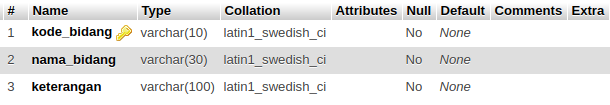
\includegraphics[width=12cm]{gambar/database/master_bidang}
                \caption{Implementasi Tabel Master Bidang}
                \label{imp_tabel_bidang}
            \end{figure}
	        \item Tabel Master Unit Kerja (\texttt{master\_unit\_kerja})
	        
	        Tabel master unit kerja ini digunakan untuk menyimpan data master unit kerja. Implementasi tabel master unit kerja dapat dilihat pada Gambar \ref{imp_tabel_unitkerja}.
	        \begin{figure}[H]
                \centering
                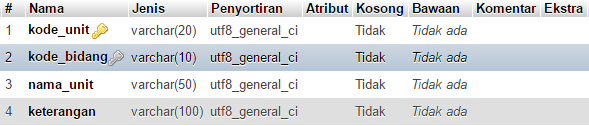
\includegraphics[width=12cm]{gambar/database/master_unit_kerja}
                \caption{Implementasi Tabel Master Unit Kerja}
                \label{imp_tabel_unitkerja}
            \end{figure}
	        \item Tabel Master Jabatan (\texttt{master\_jabatan})
	        
	        Tabel master jabatan ini digunakan untuk menyimpan data master jabatan. Implementasi tabel master jabatan dapat dilihat pada Gambar \ref{imp_tabel_jabatan}.
	        \begin{figure}[H]
                \centering
                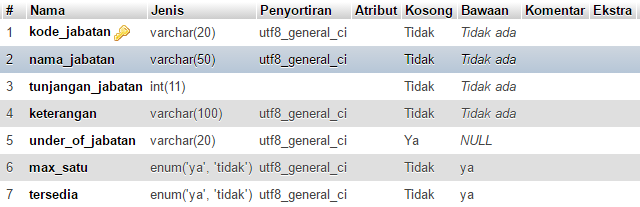
\includegraphics[width=12cm]{gambar/database/master_jabatan}
                \caption{Implementasi Tabel Master Jabatan}
                \label{imp_tabel_jabatan}
            \end{figure}
	        \item Tabel Master Periode Kerja (\texttt{master\_periode})
	        
	        Tabel master periode kerja ini digunakan untuk menyimpan data master periode kerja. Implementasi tabel master periode kerja dapat dilihat pada Gambar \ref{imp_tabel_periode}.
	        \begin{figure}[H]
                \centering
                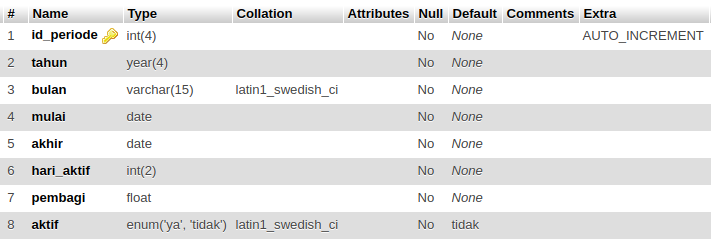
\includegraphics[width=12cm]{gambar/database/master_periode}
                \caption{Implementasi Tabel Master Periode Kerja}
                \label{imp_tabel_periode}
            \end{figure}
            \newpage
            \item Tabel Master Jam Kerja (\texttt{master\_jam\_kerja})
	        
	        Tabel master jam kerja ini digunakan untuk menyimpan data master jam kerja karyawan. Implementasi tabel master jam kerja dapat dilihat pada Gambar \ref{imp_tabel_jamkerja}.
	        \begin{figure}[H]
                \centering
                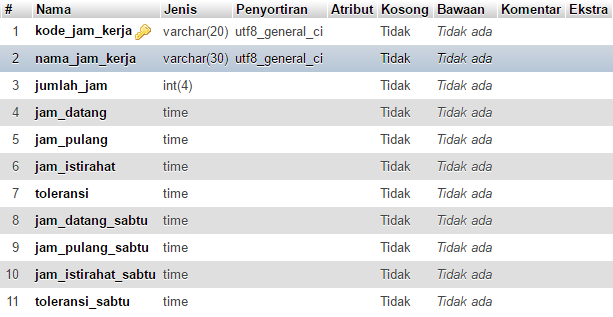
\includegraphics[width=12cm]{gambar/database/master_jam_kerja}
                \caption{Implementasi Tabel Master Jam Kerja}
                \label{imp_tabel_jamkerja}
            \end{figure}
            \item Tabel Master Program Studi (\texttt{master\_prodi})
	        
	        Tabel master program studi ini digunakan untuk menyimpan data master program studi. Implementasi tabel master program studi dapat dilihat pada Gambar \ref{imp_tabel_prodi}.
	        \begin{figure}[H]
                \centering
                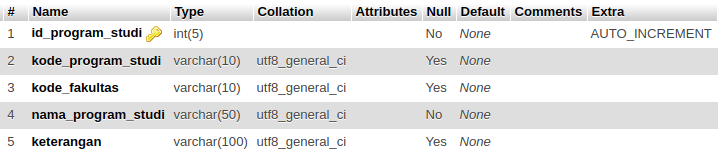
\includegraphics[width=12cm]{gambar/database/master_prodi}
                \caption{Implementasi Tabel Master Program Studi}
                \label{imp_tabel_prodi}
            \end{figure}
            \item Tabel Master Mata Kuliah (\texttt{master\_matakuliah})
	        
	        Tabel master mata kuliah ini digunakan untuk menyimpan daftar-daftar mata kuliah. Implementasi tabel master mata kuliah dapat dilihat pada Gambar \ref{imp_tabel_makul}.
	        \begin{figure}[H]
                \centering
                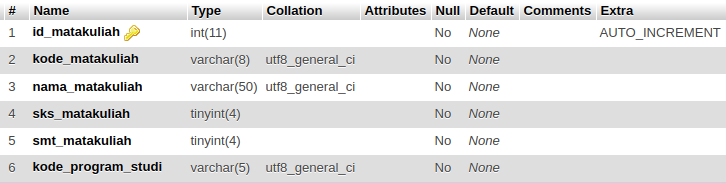
\includegraphics[width=12cm]{gambar/database/master_matakuliah}
                \caption{Implementasi Tabel Master Mata Kuliah}
                \label{imp_tabel_makul}
            \end{figure}
	        \item Tabel Master Nominal (\texttt{master\_nominal})
	        
	        Tabel master nominal ini digunakan untuk menyimpan data master nominal dari komponen-komponen penggajian. Implementasi tabel master nominal dapat dilihat pada Gambar \ref{imp_tabel_nominal}.
	        \begin{figure}[H]
                \centering
                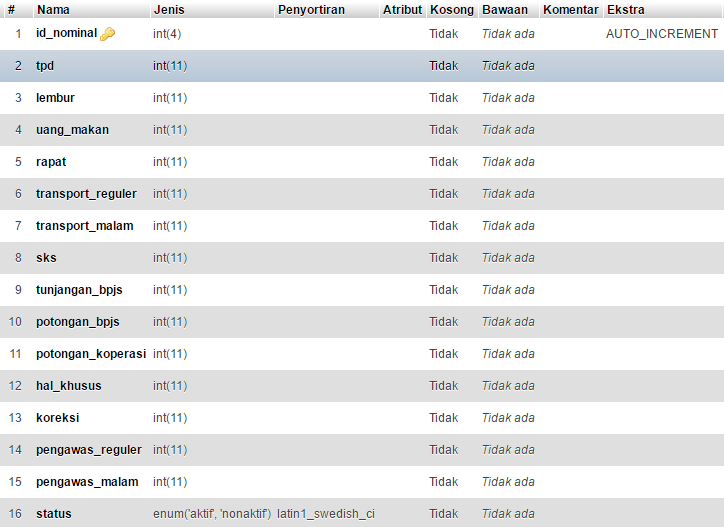
\includegraphics[width=12cm]{gambar/database/master_nominal}
                \caption{Implementasi Tabel Master Nominal}
                \label{imp_tabel_nominal}
            \end{figure}
	        \item Tabel Data Karyawan (\texttt{data\_karyawan})
	        
	        Tabel data karyawan ini digunakan untuk menyimpan data karyawan seperti nama karyawan, \emph{username}, \emph{password} dan lain-lain. Implementasi tabel data karyawan dapat dilihat pada Gambar \ref{imp_tabel_pegawai}.
	        \begin{figure}[H]
                \centering
                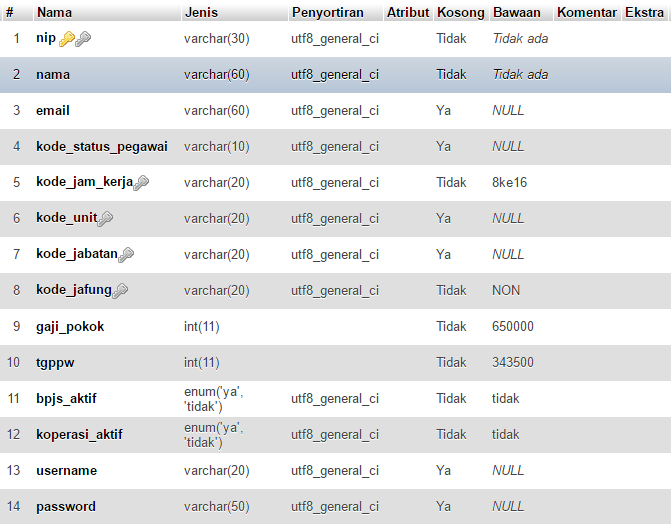
\includegraphics[width=12cm]{gambar/database/data_karyawan}
                \caption{Implementasi Tabel Data Karyawan}
                \label{imp_tabel_pegawai}
            \end{figure}
	        \item Tabel Data Absensi (\texttt{absensi\_data})
	        
	        Tabel data absensi ini digunakan untuk menyimpan data absensi dari masing-masing karyawan. Implementasi tabel data absensi dapat dilihat pada Gambar \ref{imp_tabel_absensi}.
	        \begin{figure}[H]
                \centering
                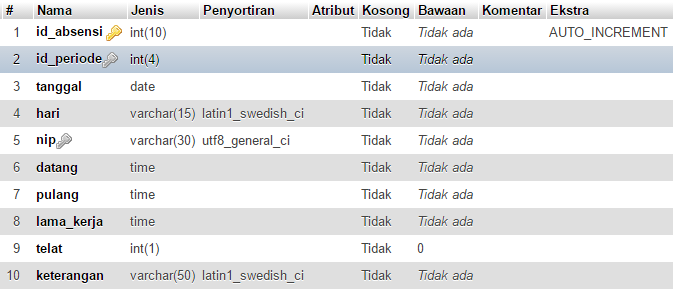
\includegraphics[width=12cm]{gambar/database/absensi_data}
                \caption{Implementasi Tabel Data Absensi}
                \label{imp_tabel_absensi}
            \end{figure}
            \newpage
	        \item Tabel Rekap Absensi (\texttt{absensi\_rekap})
	        
	        Tabel rekap absensi ini digunakan untuk menyimpan data rekap absensi karyawan. Implementasi tabel rekap absensi dapat dilihat pada Gambar \ref{imp_tabel_absensi_rekap}.
	        \begin{figure}[H]
                \centering
                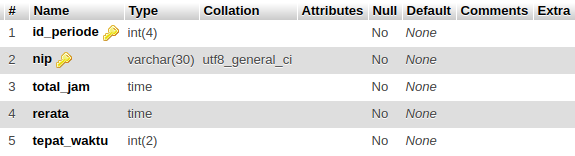
\includegraphics[width=12cm]{gambar/database/absensi_rekap}
                \caption{Implementasi Tabel Rekap Absensi}
                \label{imp_tabel_absensi_rekap}
            \end{figure}
	        \item Tabel Data Lembur (\texttt{data\_lembur})
	        
	        Tabel data lembur ini digunakan untuk menyimpan data lembur yang dilakukan karyawan. Implementasi tabel data lembur dapat dilihat pada Gambar \ref{imp_tabel_lembur}.
	        \begin{figure}[H]
                \centering
                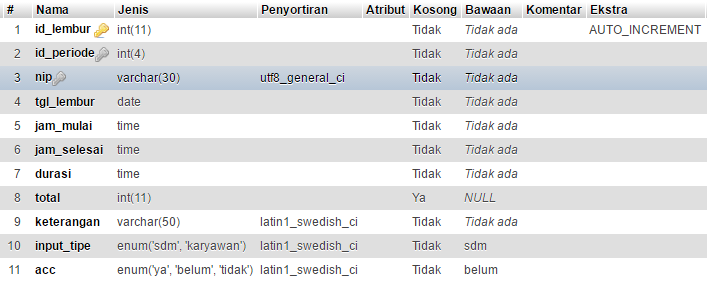
\includegraphics[width=12cm]{gambar/database/data_lembur}
                \caption{Implementasi Tabel Data Lembur}
                \label{imp_tabel_lembur}
            \end{figure}
	        \item Tabel Data Upah Lembur (\texttt{data\_upah\_lembur})
	        
	        Tabel data upah lembur ini digunakan untuk menyimpan data upah lembur yang dilakukan karyawan. Implementasi tabel data upah lembur dapat dilihat pada Gambar \ref{imp_tabel_upah_lembur}.
	        \begin{figure}[H]
                \centering
                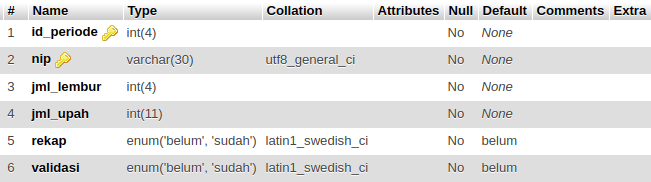
\includegraphics[width=12cm]{gambar/database/data_upah_lembur}
                \caption{Implementasi Tabel Data Upah Lembur}
                \label{imp_tabel_upah_lembur}
            \end{figure}
	        \item Tabel Data Rapat (\texttt{data\_rapat})
	        
	        Tabel data rapat ini digunakan untuk menyimpan data rapat. Implementasi tabel data rapat dapat dilihat pada Gambar \ref{imp_tabel_rapat}.
	        \begin{figure}[H]
                \centering
                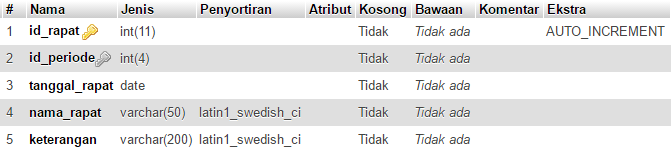
\includegraphics[width=12cm]{gambar/database/data_rapat}
                \caption{Implementasi Tabel Data Rapat}
                \label{imp_tabel_rapat}
            \end{figure}
	        \item Tabel Data Peserta Rapat (\texttt{data\_rapat\_peserta})
	        
	        Tabel data peserta rapat ini digunakan untuk menyimpan data karyawan yang mengikuti rapat. Implementasi tabel peserta rapat dapat dilihat pada Gambar \ref{imp_tabel_rapat_peserta}.
	        \begin{figure}[H]
                \centering
                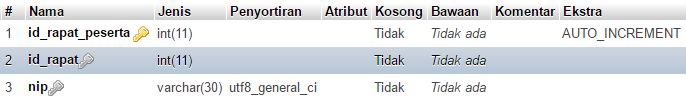
\includegraphics[width=12cm]{gambar/database/data_rapat_peserta}
                \caption{Implementasi Tabel Data Peserta Rapat}
                \label{imp_tabel_rapat_peserta}
            \end{figure}
	        \item Tabel Data Upah Rapat (\texttt{data\_upah\_rapat})
	        
	        Tabel data upah rapat ini digunakan untuk menyimpan data upah karyawan yang mengikuti rapat. Implementasi tabel data upah rapat dapat dilihat pada Gambar \ref{imp_tabel_upah_rapat}.
	        \begin{figure}[H]
                \centering
                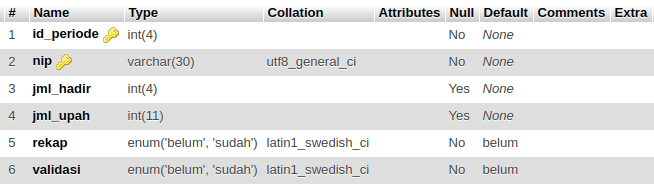
\includegraphics[width=12cm]{gambar/database/data_upah_rapat}
                \caption{Implementasi Tabel Data Upah Rapat}
                \label{imp_tabel_upah_rapat}
            \end{figure}
	        \item Tabel Data Ujian (\texttt{data\_ujian})
	        
	        Tabel data ujian ini digunakan untuk menyimpan data ujian, baik itu UTS maupun UAS. Implementasi tabel data ujian dapat dilihat pada Gambar \ref{imp_tabel_ujian}.
	        \begin{figure}[H]
                \centering
                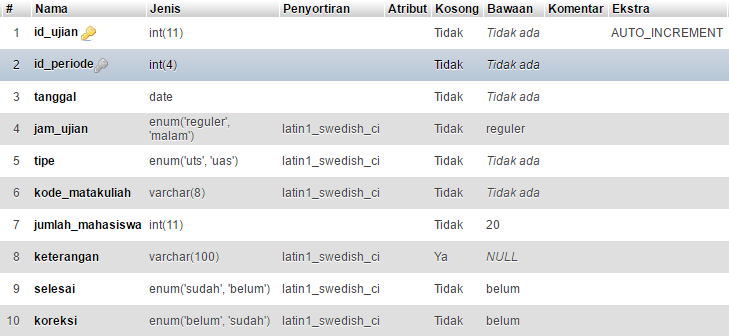
\includegraphics[width=12cm]{gambar/database/data_ujian}
                \caption{Implementasi Tabel Data Ujian}
                \label{imp_tabel_ujian}
            \end{figure}
            \item Tabel Data Pengawas Ujian (\texttt{data\_ujian\_pengawas})
            
            Tabel data pengawas ujian ini digunakan untuk menyimpan data karyawan yang menjadi pengawas ujian. Implementasi tabel data pengawas ujian dapat dilihat pada Gambar \ref{imp_tabel_ujian_pengawas}.
            \begin{figure}[H]
                \centering
                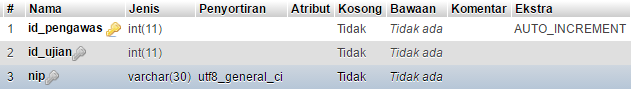
\includegraphics[width=12cm]{gambar/database/data_ujian_pengawas}
                \caption{Implementasi Tabel Data Pengawas Ujian}
                \label{imp_tabel_ujian_pengawas}
            \end{figure}
            \newpage
            \item Tabel Data Korektor Ujian (\texttt{data\_ujian\_korektor})
            
            Tabel data korektor ujian ini digunakan untuk menyimpan data karyawan yang menjadi korektor hasil ujian. Implementasi tabel data korektor ujian dapat dilihat pada Gambar \ref{imp_tabel_ujian_korektor}.
            \begin{figure}[H]
                \centering
                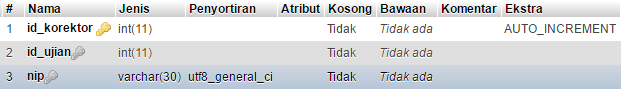
\includegraphics[width=12cm]{gambar/database/data_ujian_korektor}
                \caption{Implementasi Tabel Data Korektor Ujian}
                \label{imp_tabel_ujian_korektor}
            \end{figure}
            \item Tabel Data Upah Pengawas Ujian (\texttt{data\_upah\_pengawas})
            
            Tabel data upah pengawas ujian ini digunakan untuk menyimpan data upah pengawas ujian. Implementasi tabel data upah pengawas ujian dapat dilihat pada Gambar \ref{imp_tabel_upah_pengawas}.
            \begin{figure}[H]
                \centering
                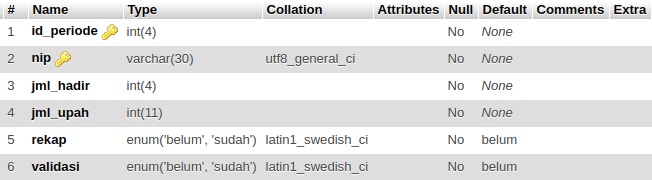
\includegraphics[width=12cm]{gambar/database/data_upah_pengawas}
                \caption{Implementasi Tabel Data Upah Pengawas}
                \label{imp_tabel_upah_pengawas}
            \end{figure}
            \item Tabel Data Upah Korektor (\texttt{data\_upah\_korektor})
            
            Tabel data upah korektor ujian ini digunakan untuk menyimpan data upah korektor ujian. Implementasi tabel data upah korektor ujian dapat dilihat pada Gambar \ref{imp_tabel_upah_korektor}.
            \begin{figure}[H]
                \centering
                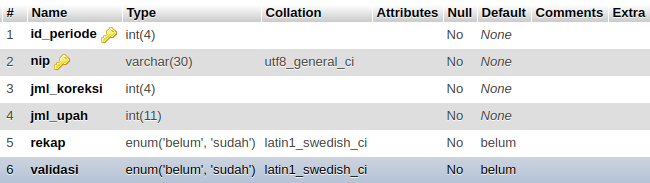
\includegraphics[width=12cm]{gambar/database/data_upah_korektor}
                \caption{Implementasi Tabel Data Upah Korektor}
                \label{imp_tabel_upah_korektor}
            \end{figure}
            \item Tabel Data Rencana dan Laporan Kerja Harian (\texttt{data\_rkhlh})
            
            Tabel data rencana dan laporan harian ini digunakan untuk menyimpan data rencana dan laporan harian masing-masing karyawan. Implementasi tabel data rencana dan laporan kerja harian dapat dilihat pada Gambar \ref{imp_tabel_rkhlh}.
            \begin{figure}[H]
                \centering
                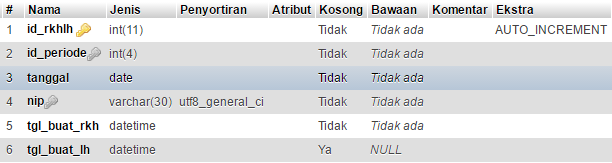
\includegraphics[width=12cm]{gambar/database/data_rkhlh}
                \caption{Implementasi Tabel Data Rencana dan Laporan Harian}
                \label{imp_tabel_rkhlh}
            \end{figure}
            \item Tabel Detail Rencana dan Laporan Kerja Harian (\texttt{data\_rkhlh\_detail})
            
            Tabel detail rencana dan laporan harian ini digunakan untuk menyimpan detail kegiatan dari masing-masing rencana dan laporan harian. Implementasi tabel detail rencana dan laporan kerja harian dapat dilihat pada Gambar \ref{imp_tabel_rkhlh_detail}.
            \begin{figure}[H]
                \centering
                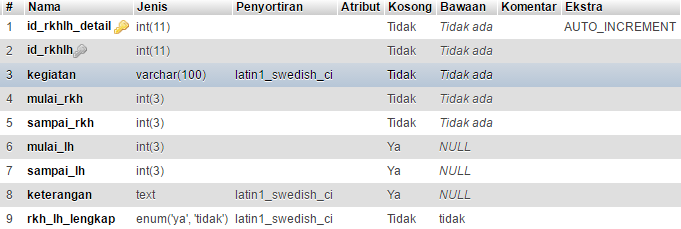
\includegraphics[width=12cm]{gambar/database/data_rkhlh_detail}
                \caption{Implementasi Tabel Detail Rencana dan Laporan Harian}
                \label{imp_tabel_rkhlh_detail}
            \end{figure}
            \item Tabel Data Checklist dan Laporan Kerja Bulanan (\texttt{data\_cblb})
            
            Tabel data checklist dan laporan bulanan ini digunakan untuk menyimpan data checklist dan laporan bulanan masing-masing karyawan. Implementasi tabel data checklist dan laporan kerja bulanan dapat dilihat pada Gambar \ref{imp_tabel_cblb}.
            \begin{figure}[H]
                \centering
                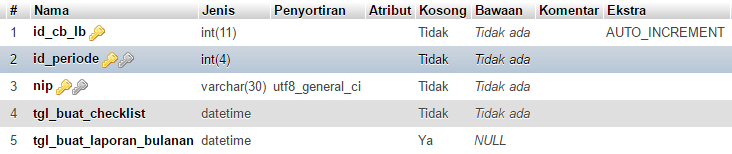
\includegraphics[width=12cm]{gambar/database/data_cblb}
                \caption{Implementasi Tabel Data Checklist dan Laporan Bulanan}
                \label{imp_tabel_cblb}
            \end{figure}
            \item Tabel Detail Checklist dan Laporan Kerja Bulanan (\texttt{data\_cblb\_detail})
            
            Tabel detail checklist dan laporan bulanan ini digunakan untuk menyimpan detail kegiatan dari masing-masing checklist dan laporan bulanan. Implementasi tabel detail checklist dan laporan kerja bulanan dapat dilihat pada Gambar \ref{imp_tabel_cblb_detail}.
            \begin{figure}[H]
                \centering
                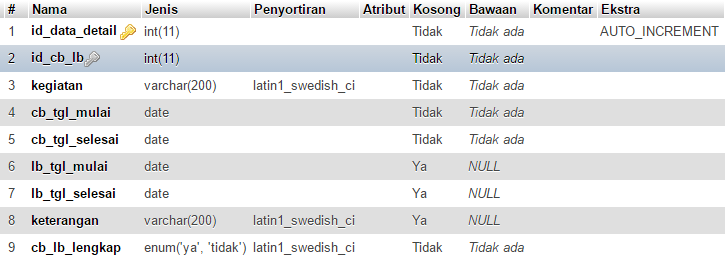
\includegraphics[width=12cm]{gambar/database/data_cblb_detail}
                \caption{Implementasi Tabel Detail Checklist dan Laporan Bulanan}
                \label{imp_tabel_cblb_detail}
            \end{figure}
            \item Tabel Data Insentif Operasional (\texttt{data\_insentif\_op})
            
            Tabel data insentif operasional ini digunakan untuk menyimpan data insentif operasional karyawan yang diinput oleh kepala unit. Implementasi tabel data insentif operasional dapat dilihat pada Gambar \ref{imp_tabel_insentif}.
            \begin{figure}[H]
                \centering
                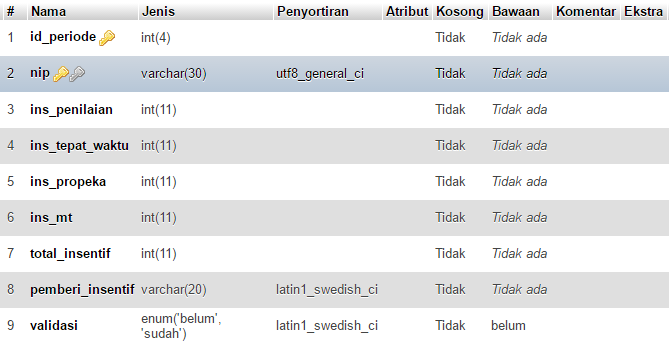
\includegraphics[width=12cm]{gambar/database/data_insentif_op}
                \caption{Implementasi Tabel Data Insentif Operasional}
                \label{imp_tabel_insentif}
            \end{figure}
            \item Tabel Data Penilaian Kinerja (\texttt{data\_penilaian})
            
            Tabel data penilaian kinerja ini digunakan untuk menyimpan data penilaian kinerja karyawan yang diinput oleh kepala unit. Implementasi tabel data penilaian kinerja dapat dilihat pada Gambar \ref{imp_tabel_penilaian}.
            \begin{figure}[H]
                \centering
                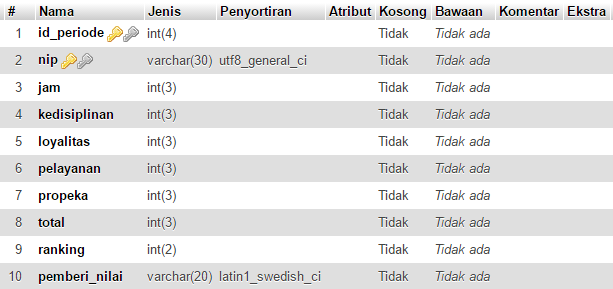
\includegraphics[width=12cm]{gambar/database/data_penilaian}
                \caption{Implementasi Tabel Data Penilaian Kinerja}
                \label{imp_tabel_penilaian}
            \end{figure}
            \item Tabel Data Slip Gaji (\texttt{data\_slip\_gaji})
            
            Tabel data slip gaji digunakan untuk menyimpan data slip gaji karyawan. Implementasi tabel data slip gaji dapat dilihat pada Gambar \ref{imp_tabel_slip}.
            \begin{figure}[H]
                \centering
                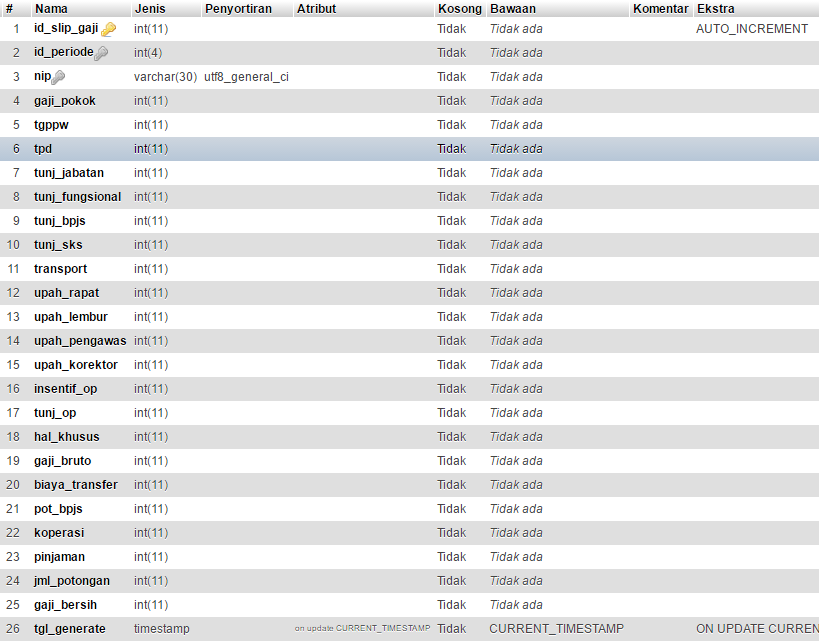
\includegraphics[width=14cm]{gambar/database/data_slip_gaji}
                \caption{Implementasi Tabel Data Slip Gaji}
                \label{imp_tabel_slip}
            \end{figure}
	    \end{enumerate}
	    
	    \subsection{Implementasi Antarmuka (\emph{Interface})}
	    Implementasi antaramuka sistem merupakan hasil dari pembuatan antarmuka sistem yang berdasarkan rancangan antarmuka yang telah peneliti lakukan sebelumnya. Peneliti menggunakan \emph{Sublime Text} sebagai \emph{text editor}. Berikut hasil implementasi antarmuka sistem yang dikembangkan:
	    \begin{enumerate}
	        \itemsep0em
	        \item Implementasi Halaman \emph{Login}
	        
	        Halaman ini digunakan untuk semua aktor (\emph{user}) ketika ingin \emph{Login} ke dalam sistem. Implementasi halaman \emph{Login} dapat dilihat pada Gambar \ref{imp_hal_login}.
	        \begin{figure}[H]
                \centering
                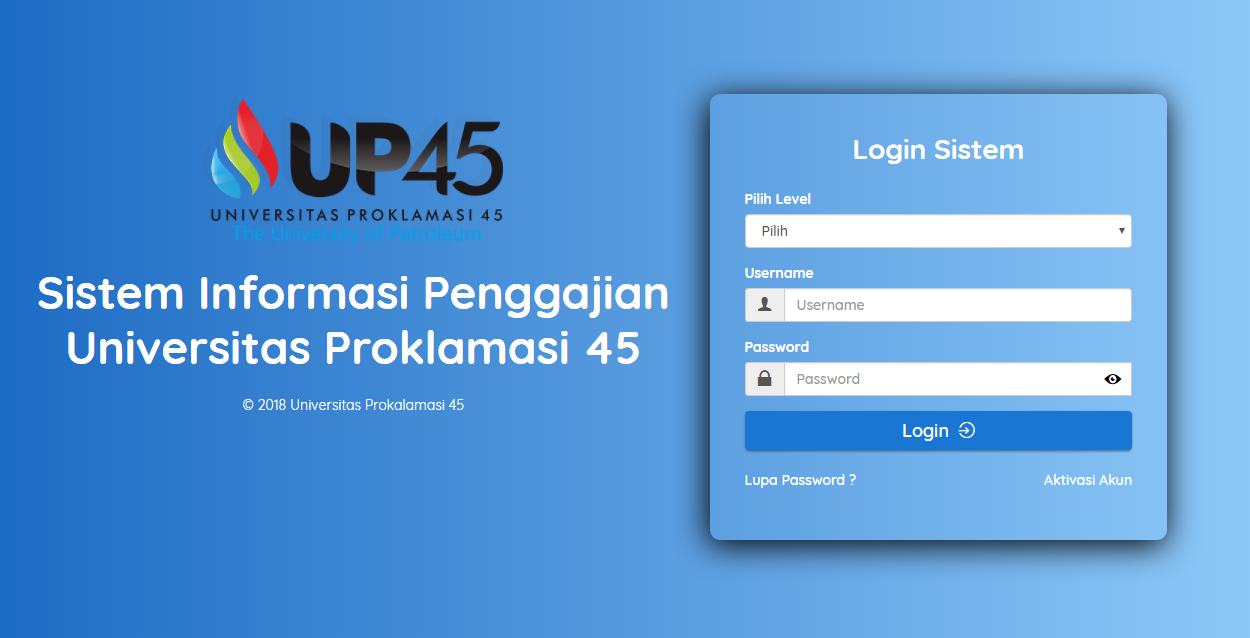
\includegraphics[width=13cm]{gambar/halaman/halaman-login}
                \caption{Implementasi Halaman Login}
                \label{imp_hal_login}
            \end{figure}
            \item Implementasi Halaman Manajemen Periode Kerja
            
            Halaman ini digunakan oleh staf SDM untuk menambah data periode kerja. Pada \emph{form} tambah periode kerja, staf SDM dapat mengisi tanggal awal periode dan tanggal akhir periode. Implementasi halaman manajemen periode kerja dapat dilihat pada Gambar \ref{imp_hal_data_periode}.
	        \begin{figure}[H]
                \centering
                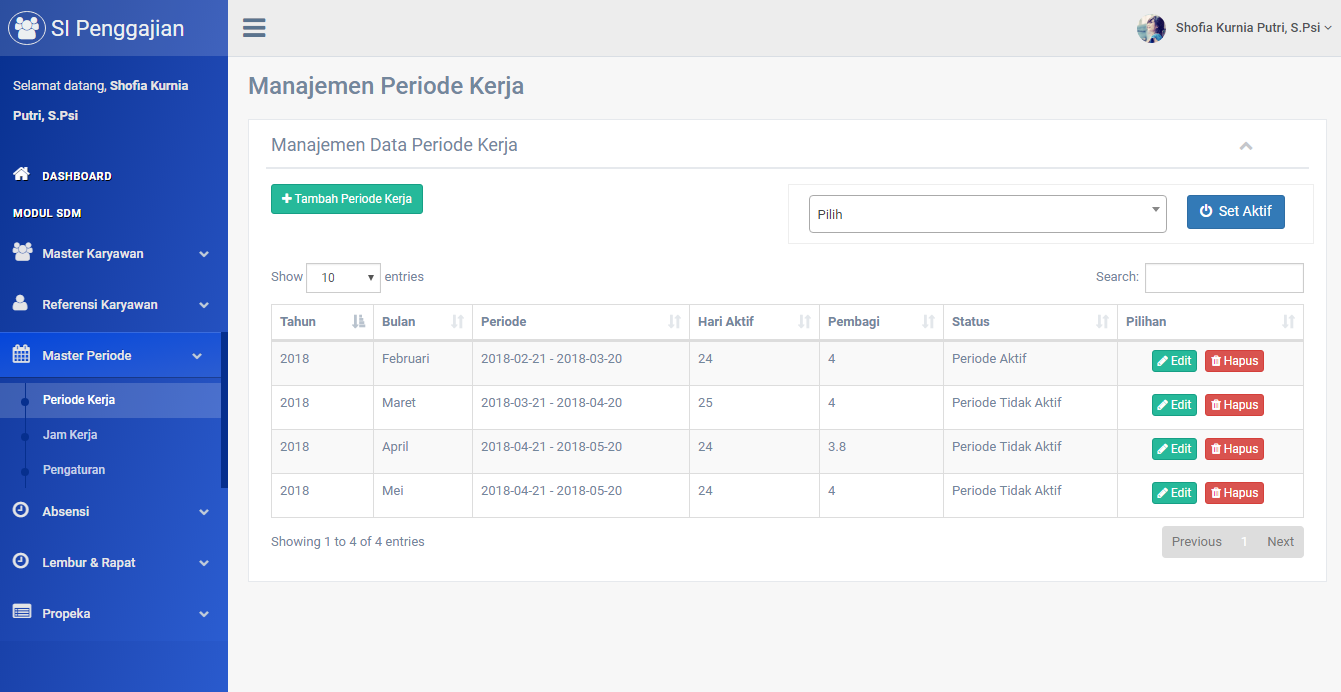
\includegraphics[width=15cm]{gambar/halaman/halaman-data-periode}
                \caption{Implementasi Halaman Manajemen Periode Kerja}
                \label{imp_hal_data_periode}
            \end{figure}
            \newpage
            \item Implementasi Halaman Manajemen Unit Kerja
            
            Pada halaman ini staf SDM dapat melihat data unit kerja, serta dapat melakukan tindakan tambah data, edit data dan hapus data. Implementasi halaman manajemen data unit kerja dapat dilihat pada Gambar \ref{imp_hal_data_unit} dan Gambar \ref{imp_hal_tambah_unit}.
	        \begin{figure}[H]
                \centering
                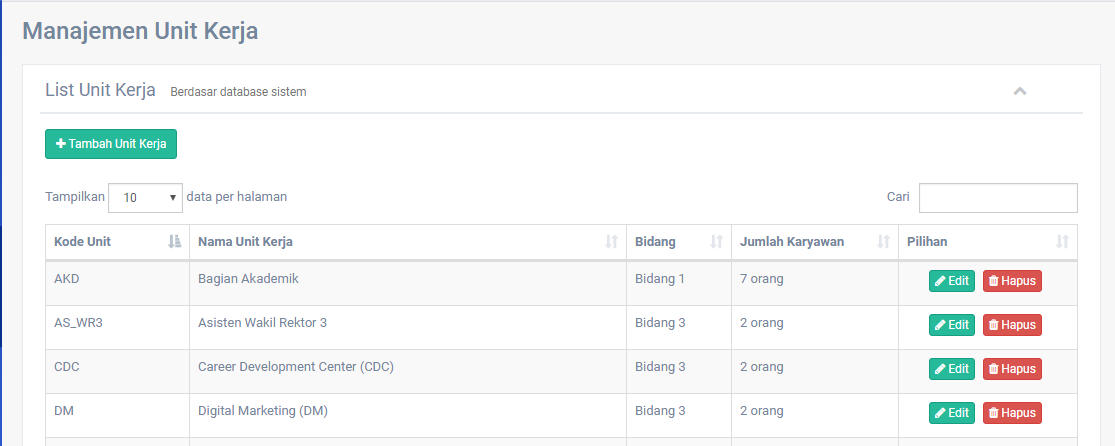
\includegraphics[width=14cm]{gambar/halaman/halaman-data-unit}
                \caption{Implementasi Halaman Data Unit Kerja}
                \label{imp_hal_data_unit}
            \end{figure}
            \begin{figure}[H]
                \centering
                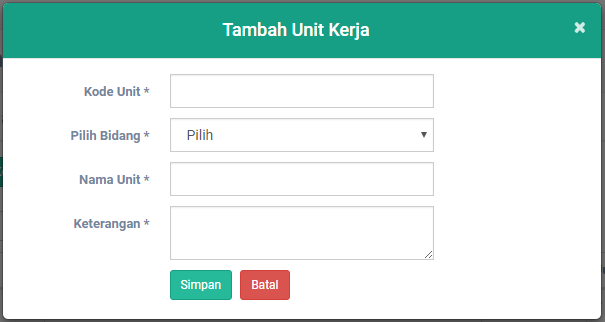
\includegraphics[width=10cm]{gambar/halaman/halaman-tambah-unit}
                \caption{Implementasi Halaman Tambah Unit Kerja}
                \label{imp_hal_tambah_unit}
            \end{figure}
            \item Implementasi Halaman Manajemen Jabatan
            
            Implementasi halaman manajemen data jabatan ini tidak jauh berbeda dengan halaman manajemen data unit kerja. Hanya saja yang ditampilkan adalah data-data jabatan.
	        \item Implementasi Halaman Manajemen Data Karyawan
	        
	        Pada halaman ini staf SDM dapat melihat data karyawan, mengubah data karyawan, mutasi karyawan dan mengubah jam kerja karyawan. Implementasi halaman manajemen data karyawan dapat dilihat pada Gambar \ref{imp_hal_data_karyawan}, Gambar \ref{imp_hal_detail_karyawan}, Gambar \ref{imp_hal_mutasi_karyawan} dan Gambar \ref{imp_hal_detail_karyawan}.
	        \begin{figure}[H]
                \centering
                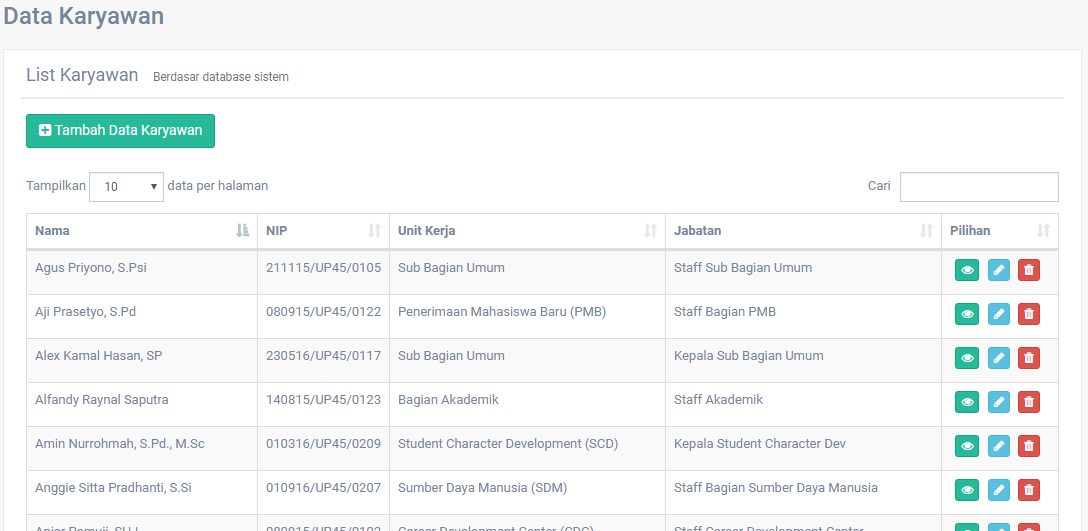
\includegraphics[width=14cm]{gambar/halaman/halaman-data-karyawan}
                \caption{Implementasi Halaman Data Karyawan}
                \label{imp_hal_data_karyawan}
            \end{figure}
            \begin{figure}[H]
                \centering
                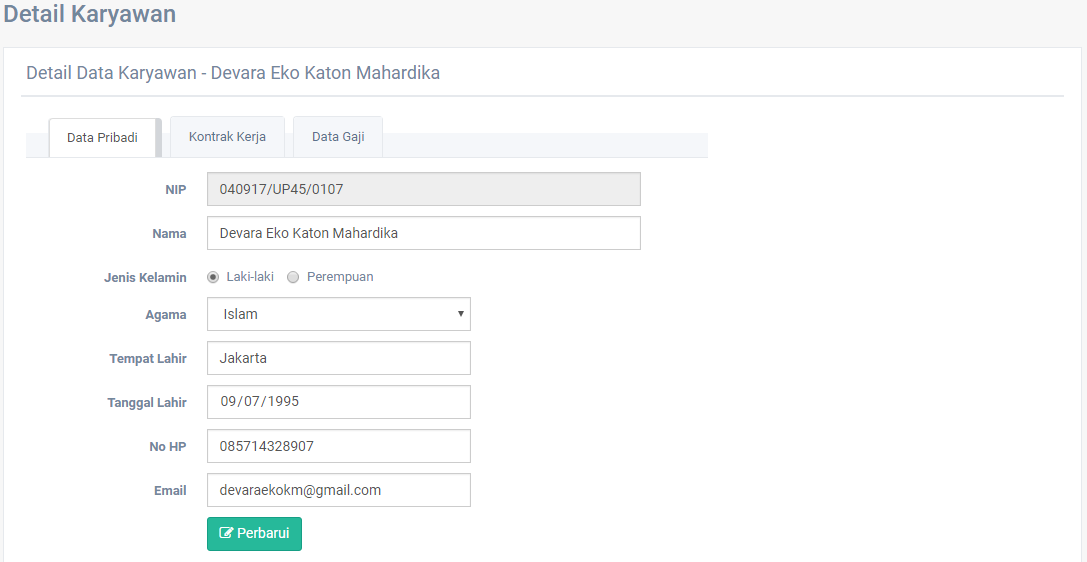
\includegraphics[width=14cm]{gambar/halaman/halaman-detail-karyawan}
                \caption{Implementasi Halaman Detail Karyawan}
                \label{imp_hal_detail_karyawan}
            \end{figure}
            \begin{figure}[H]
                \centering
                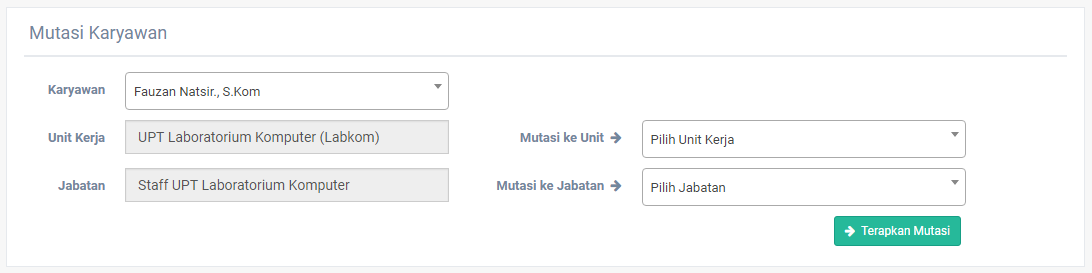
\includegraphics[width=14cm]{gambar/halaman/halaman-mutasi}
                \caption{Implementasi Halaman Mutasi Karyawan}
                \label{imp_hal_mutasi_karyawan}
            \end{figure}
            \item Implementasi Halaman Manajemen Absensi
            
            Dalam melakukan proses manajemen data absensi, terdapat beberapa halaman diantaranya adalah halaman data absensi, halaman \emph{upload} data absensi dan halaman ubah data absensi. Implementasi halaman tersebut dapat dilihat pada Gambar \ref{imp_hal_data_absensi}, Gambar \ref{imp_hal_upload_absensi}, dan Gambar \ref{imp_hal_ubah_absensi}.
	        \begin{figure}[H]
                \centering
                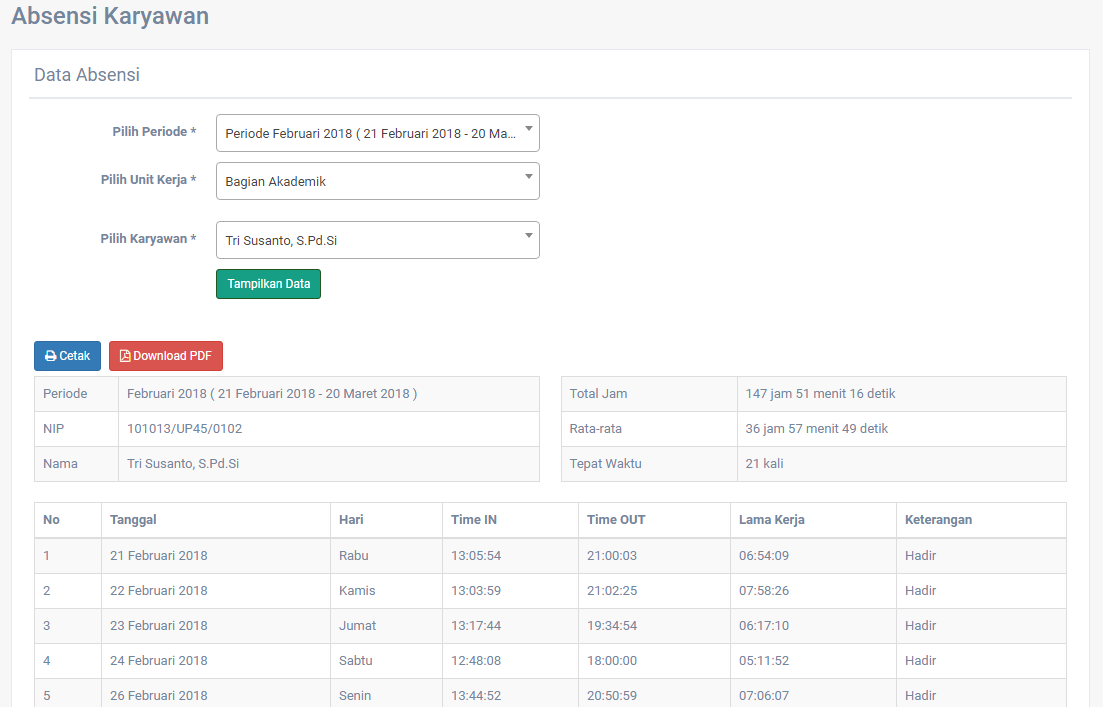
\includegraphics[width=15cm]{gambar/halaman/halaman-data-absensi}
                \caption{Implementasi Halaman Data Absensi}
                \label{imp_hal_data_absensi}
            \end{figure}
            \begin{figure}[H]
                \centering
                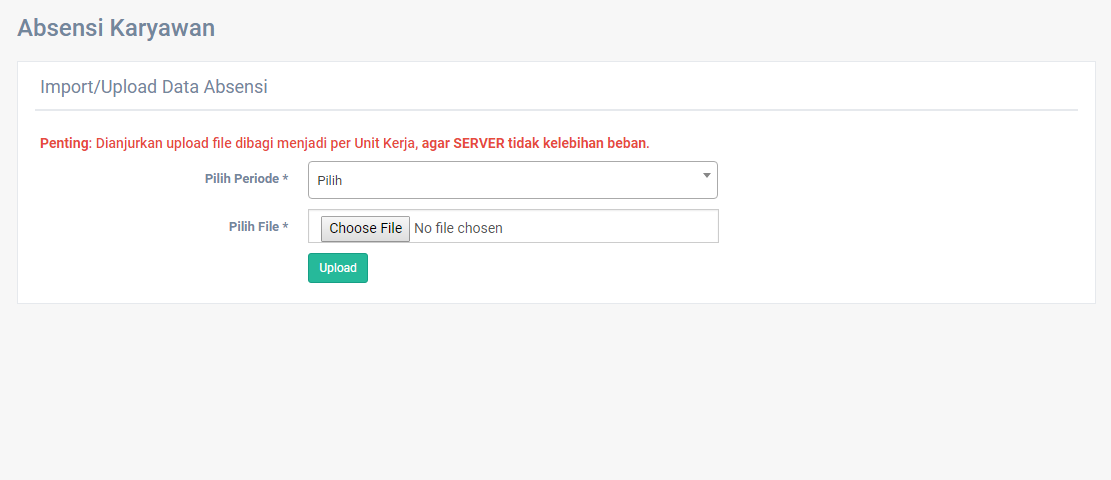
\includegraphics[width=13cm]{gambar/halaman/halaman-upload-absensi}
                \caption{Implementasi Halaman \emph{Upload} Absensi}
                \label{imp_hal_upload_absensi}
            \end{figure}
            \begin{figure}[H]
                \centering
                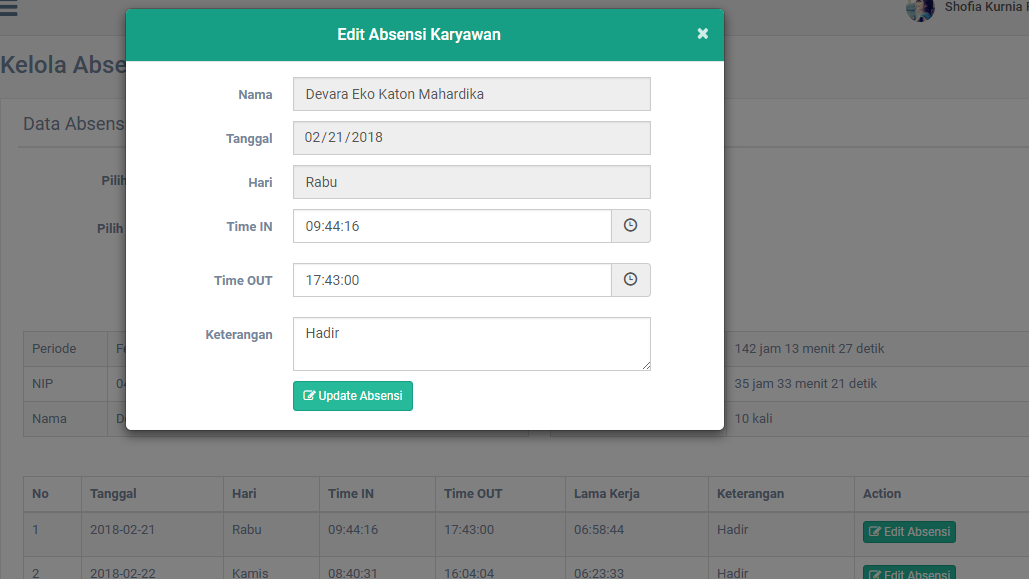
\includegraphics[width=14cm]{gambar/halaman/halaman-kelola-absensi}
                \caption{Implementasi Halaman Ubah Absensi}
                \label{imp_hal_ubah_absensi}
            \end{figure}
            \item Implementasi Halaman Manajemen Lembur
            
            Dalam melakukan proses manajemen data lembur, terdapat beberapa halaman diantaranya adalah halaman data lembur dan halaman tambah data lembur yang menyediakan \emph{form} untuk input data lembur seperti jam lembur serta karyawan yang melakukan lembur. Implementasi halaman tersebut dapat dilihat pada Gambar \ref{imp_hal_data_lembur} dan Gambar \ref{imp_hal_tambah_lembur}.
	        \begin{figure}[H]
                \centering
                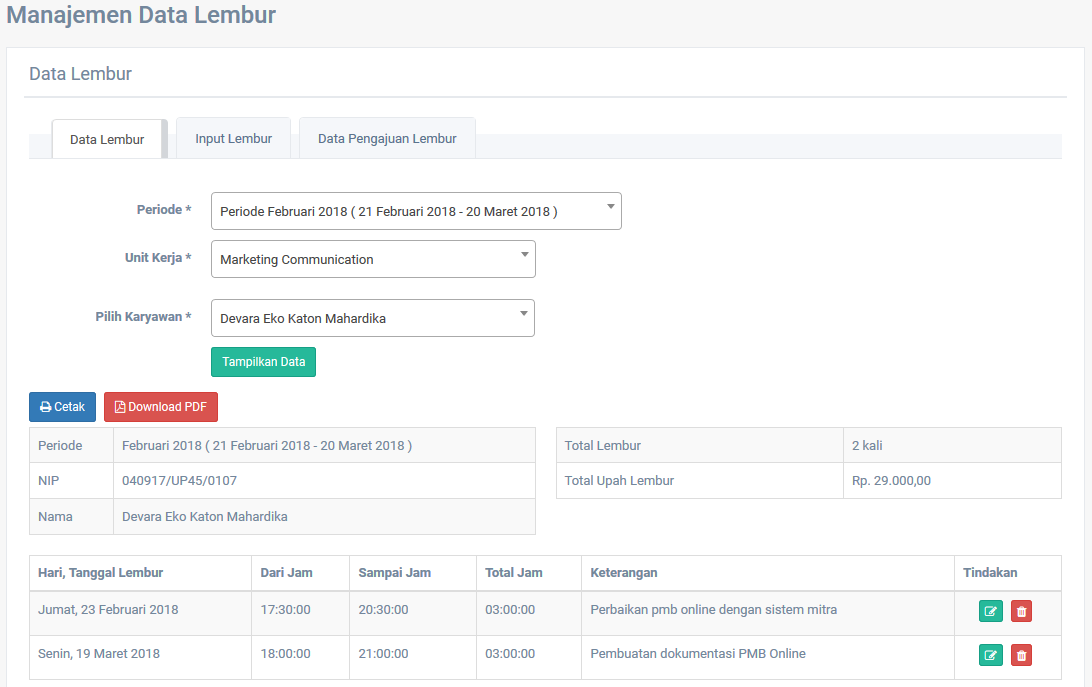
\includegraphics[width=13cm]{gambar/halaman/halaman-data-lembur}
                \caption{Implementasi Halaman Data Lembur}
                \label{imp_hal_data_lembur}
            \end{figure}
            \begin{figure}[H]
                \centering
                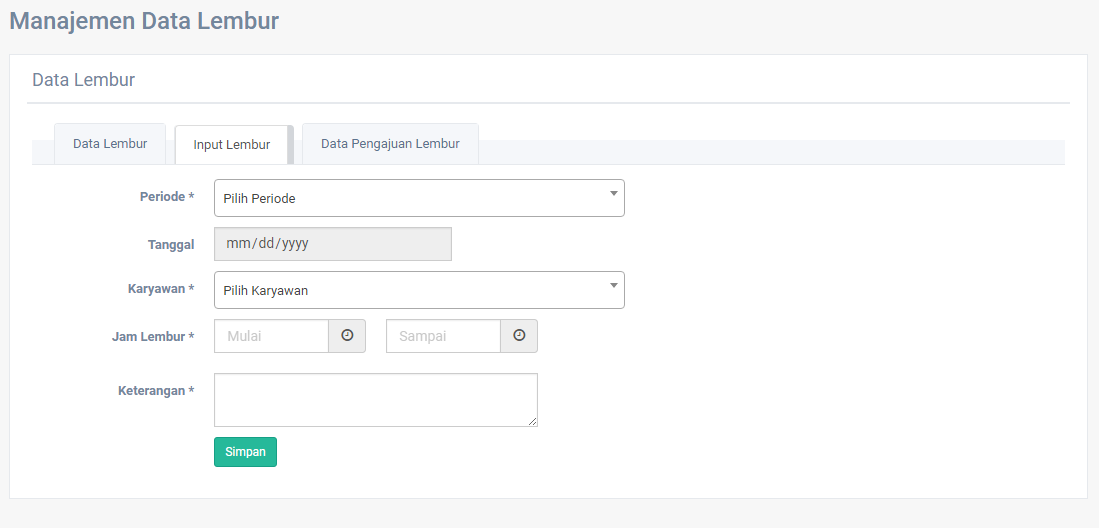
\includegraphics[width=13cm]{gambar/halaman/halaman-tambah-lembur}
                \caption{Implementasi Halaman Tambah Lembur}
                \label{imp_hal_tambah_lembur}
            \end{figure}
            \item Implementasi Halaman Manajemen Rapat
            
            Dalam melakukan proses manajemen data rapat, terdapat beberapa halaman diantaranya adalah halaman data rapat dan halaman tambah data rapat yang menyediakan \emph{form} untuk input data rapat seperti tanggal rapat serta karyawan yang menjadi peserta rapat. Implementasi halaman tersebut dapat dilihat pada Gambar \ref{imp_hal_data_rapat} dan Gambar \ref{imp_hal_tambah_rapat}.
	        \begin{figure}[H]
                \centering
                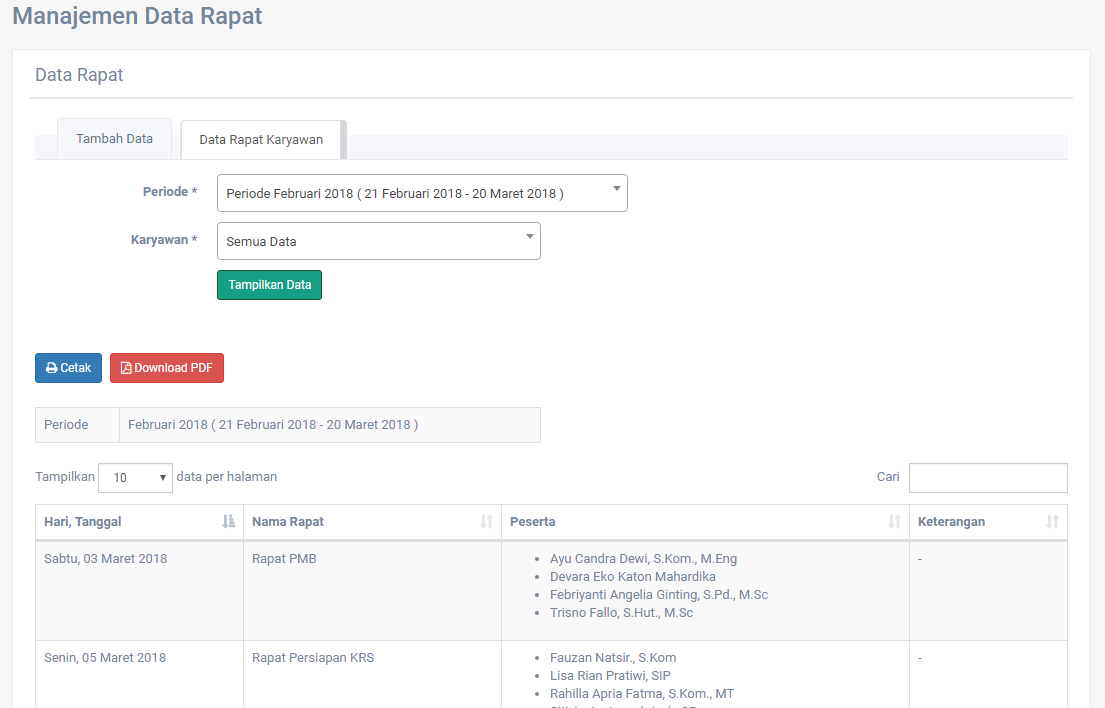
\includegraphics[width=14cm]{gambar/halaman/halaman-data-rapat}
                \caption{Implementasi Halaman Data Rapat}
                \label{imp_hal_data_rapat}
            \end{figure}
            \begin{figure}[H]
                \centering
                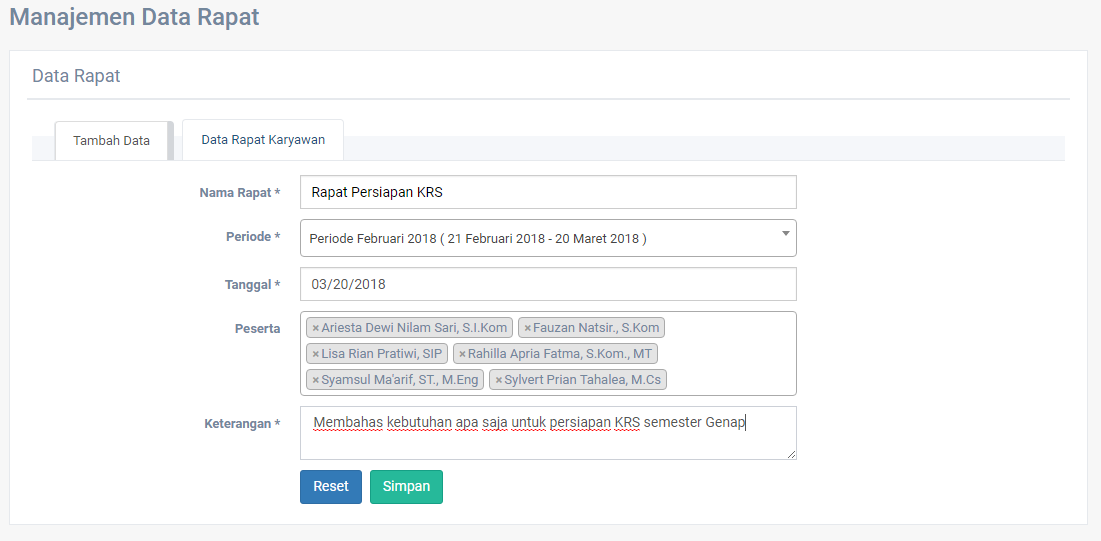
\includegraphics[width=14cm]{gambar/halaman/halaman-tambah-rapat}
                \caption{Implementasi Halaman Tambah Rapat}
                \label{imp_hal_tambah_rapat}
            \end{figure}
            \newpage
            \item Implementasi Halaman Manajemen Laporan Kerja Karyawan
            
            Halaman ini digunakan untuk melakukan manajemen laporan kerja, seperti tambah rencana kerja harian dan laporan kerja harian untuk aktor karyawan. Kepala unit menggunakan halaman ini untuk melihat laporan kerja karyawan yang dibawahinya. Implementasi halaman tersebut dapat dilihat pada Gambar \ref{imp_hal_tambah_rkh}, Gambar \ref{imp_hal_tambah_lh}, Gambar \ref{imp_hal_data_rkhlh}, dan Gambar \ref{imp_hal_lihat_lh}.
            \begin{figure}[H]
                \centering
                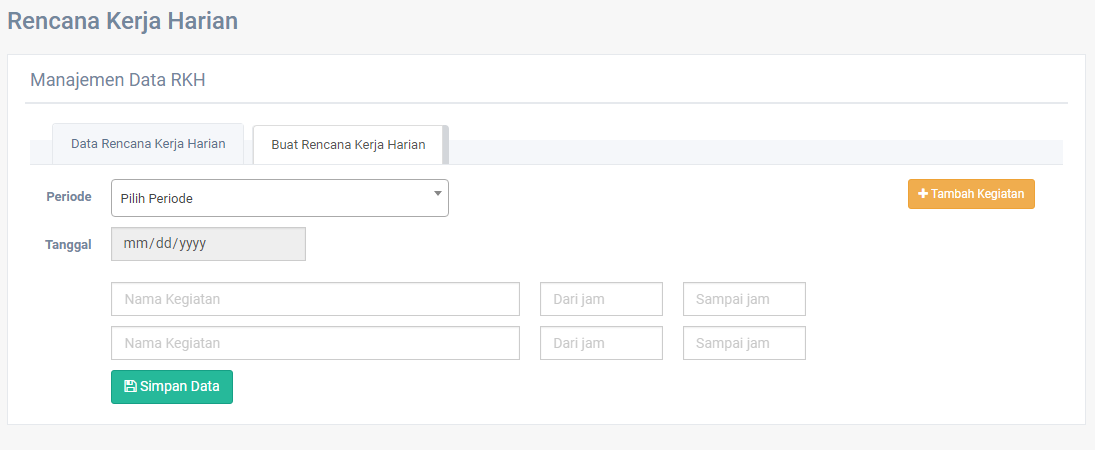
\includegraphics[width=14cm]{gambar/halaman/halaman-tambah-rkh}
                \caption{Implementasi Halaman Tambah Rencana Kerja Harian}
                \label{imp_hal_tambah_rkh}
            \end{figure}
            \begin{figure}[H]
                \centering
                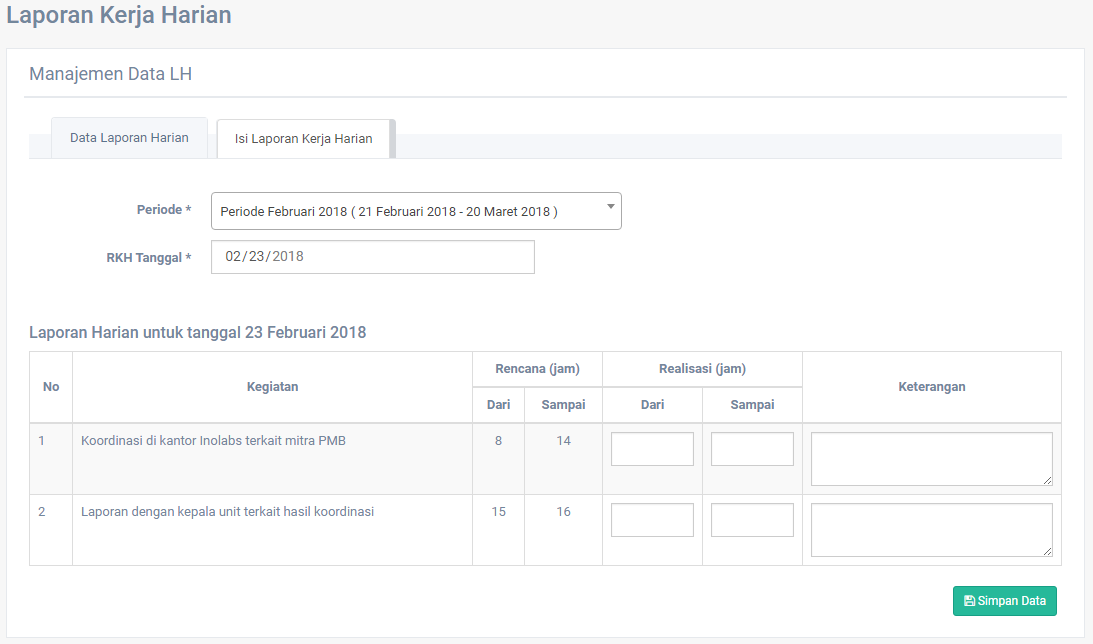
\includegraphics[width=14cm]{gambar/halaman/halaman-tambah-lh}
                \caption{Implementasi Halaman Tambah Laporan Kerja Harian}
                \label{imp_hal_tambah_lh}
            \end{figure}
            \begin{figure}[H]
                \centering
                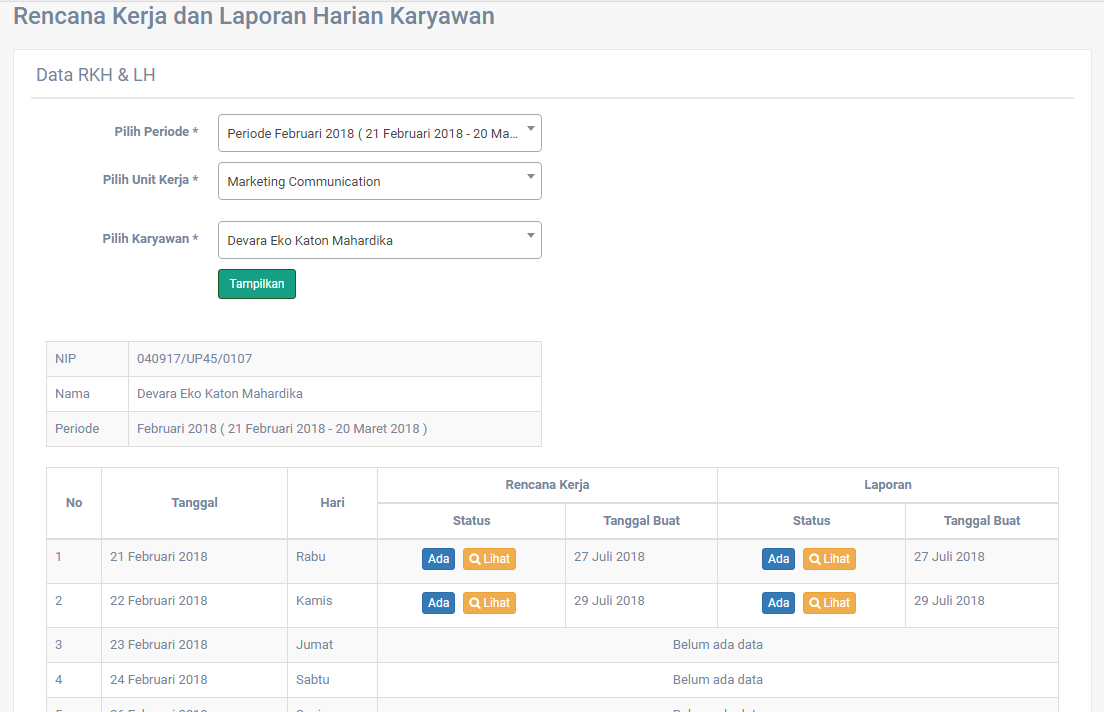
\includegraphics[width=15cm]{gambar/halaman/halaman-data-rkhlh}
                \caption{Implementasi Halaman Data Laporan Kerja Harian}
                \label{imp_hal_data_rkhlh}
            \end{figure}
            \begin{figure}[H]
                \centering
                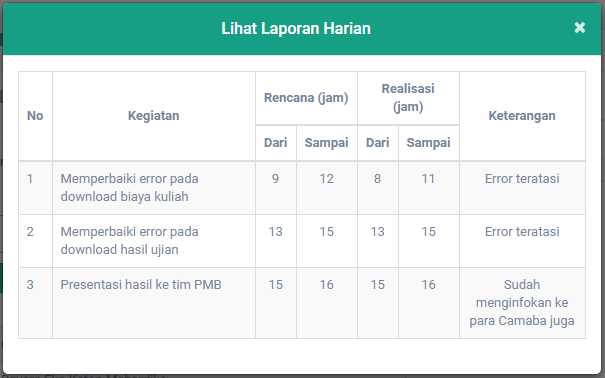
\includegraphics[width=11cm]{gambar/halaman/halaman-lihat-lh}
                \caption{Implementasi Halaman Lihat Laporan Kerja Harian}
                \label{imp_hal_lihat_lh}
            \end{figure}
            \item Implementasi Halaman Manajemen Slip Gaji
            
            Halaman ini digunakan untuk melakukan proses \emph{generate} slip gaji karyawan dan melihat data slip gaji karyawan. Implementasi kedua halaman tersebut dapat dilihat pada Gambar \ref{imp_hal_generate_slip} dan Gambar \ref{imp_hal_data_slip}.
	        \begin{figure}[H]
                \centering
                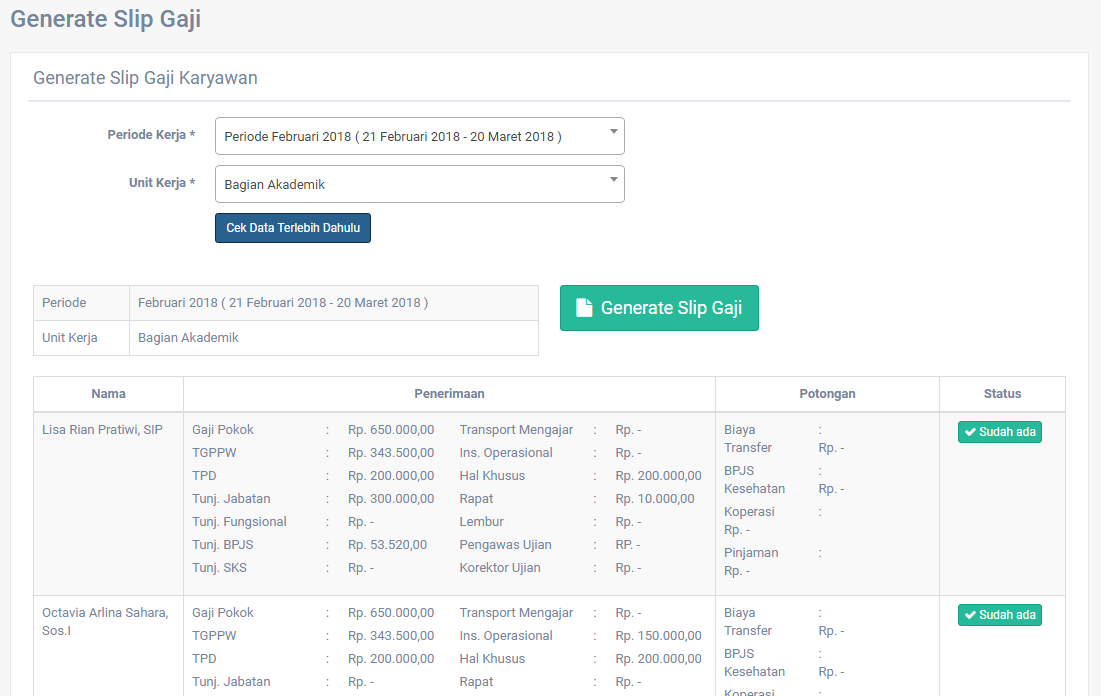
\includegraphics[width=15cm]{gambar/halaman/halaman-generate-slip}
                \caption{Implementasi Halaman Generate Slip}
                \label{imp_hal_generate_slip}
            \end{figure}
            \begin{figure}[H]
                \centering
                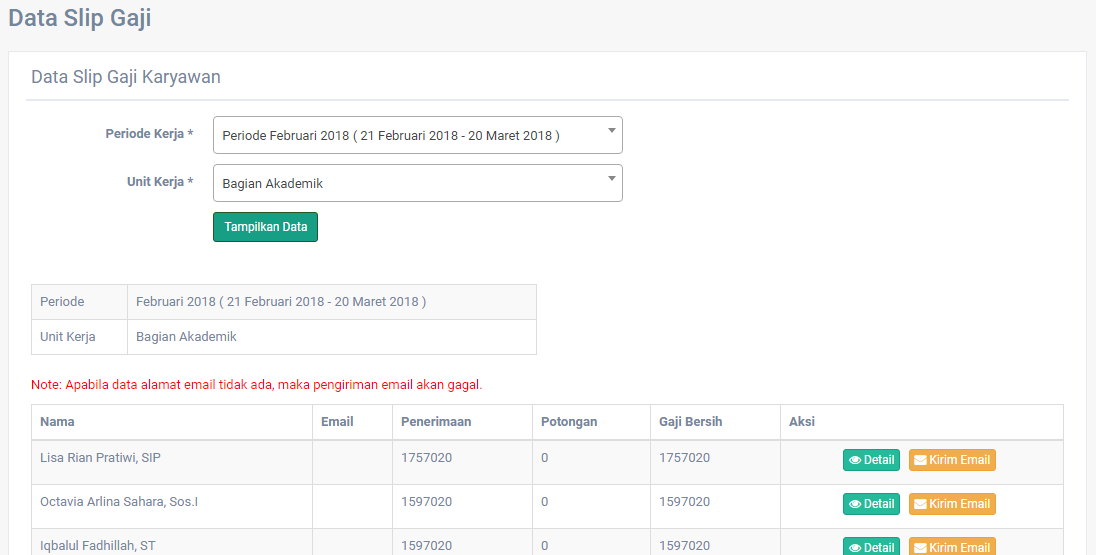
\includegraphics[width=14cm]{gambar/halaman/halaman-data-slip}
                \caption{Implementasi Halaman Data Slip}
                \label{imp_hal_data_slip}
            \end{figure}
	    \end{enumerate}
	    
	\section{\emph{Testing} (Pengujian Sistem)}
	Pengujian sistem merupakan tahapan terakhir dalam pengembangan sistem ini. Tujuan dari pengujian ini adalah untuk memastikan bahwa fitur dalam sistem yang dikembangkan dapat berfungsi sesuai yang diharapkan.
	
	    \subsection{Pengujian \emph{Alpha}}
	    Pengujian \emph{alpha} dilakukan oleh peneliti selaku pengembang sistem bersama dengan pihak Universitas Proklamasi 45 selaku \emph{project owner}. Tujuan dari pengujian \emph{alpha} adalah untuk melakukan uji fungsionalitas dari sistem apakah sudah berjalan dengan baik atau tidak. Detail dari pengujian ini dapat dilihat pada Tabel \ref{tabel_pengujian_alpha}.
	    \begin{spacing}{1.25}
	    \begin{longtable}{|>{\centering}p{1.5em}|>{\raggedright}p{3cm}|>{\raggedright}p{6.5cm}|p{2cm}|}
    	    \caption{Pengujian \emph{Alpha}} 
	        \label{tabel_pengujian_alpha} \\
            \hline
            \textbf{No.} & \centering \textbf{Item Uji} & \centering \textbf{Detail Pengujian} & \textbf{Jenis Uji} \\
            \hline 
            \endfirsthead
                        
            \multicolumn{4}{c}{{\bfseries \tablename\ \thetable{}: }Pengujian \emph{Alpha} (lanjutan)} \\
            \hline
            \textbf{No.} & \centering \textbf{Item Uji} & \centering \textbf{Detail Pengujian} & \textbf{Jenis Uji} \\ \hline
            \endhead
            \hline
            \endfoot
            \hline \hline
            \endlastfoot
    	    
    	    \multirow{2}{*}{1.} & \multirow{2}{3cm}{Login Sistem} & Menampilkan pesan kesahalahan ketika hak akses tidak sesuai & \multirow{2}{*}{Black box} \\ \cline{3-3}
    	    & & Menampilkan halaman dashboard sesuai hak akses ketika berhasil login & \\ \hline
    	    \multirow{4}{*}{2.} & \multirow{3}{3cm}{Manajemen Periode Kerja} & Menampilkan data periode kerja & \multirow{3}{*}{Black box} \\ \cline{3-3}
    	    & & Menambah periode kerja & \\ \cline{3-3}
    	    & & Mengatur periode kerja yang sedang aktif & \\ \cline{3-3}
    	    & & Menampilkan pesan sukses/error tambah periode kerja & \\ \hline
    	    \multirow{6}{*}{3.} & \multirow{5}{3cm}{Manajemen Data Unit Kerja} & Menampilkan data unit kerja & \multirow{5}{*}{Black box} \\ \cline{3-3}
    	    & & Menambah data unit kerja & \\ \cline{3-3}
    	    & & Mengubah data unit kerja & \\ \cline{3-3}
    	    & & Menghapus data unit kerja & \\ \cline{3-3}
    	    & & Menampilkan pesan sukses/error ketika tambah dan edit unit kerja & \\ \cline{3-3}
    	    & & Menampilkan pesan error ketika hapus unit kerja yang terisi oleh karyawan & \\ \hline
    	    \multirow{6}{*}{4.} & \multirow{5}{3cm}{Manajemen Data Jabatan} & Menampilkan data jabatan & \multirow{5}{2cm}{Black box} \\ \cline{3-3}
    	    & & Menambah data jabatan & \\ \cline{3-3}
    	    & & Mengubah data jabatan & \\ \cline{3-3}
    	    & & Menghapus data jabatan & \\ \cline{3-3}
    	    & & Menampilkan pesan sukses/error ketika tambah dan edit jabatan & \\ \cline{3-3}
    	    & & Menampilkan pesan error ketika hapus jabatan yang terisi oleh karyawan & \\ \hline
    	    \multirow{6}{*}{5.} & \multirow{4}{3cm}{Manajemen Karyawan} & Menampilkan data karyawan & \multirow{4}{*}{Black box} \\ \cline{3-3}
    	    & & Menambah data karyawan & \\ \cline{3-3}
    	    & & Mengubah data karyawan tertentu & \\ \cline{3-3}
    	    & & Menghapus data karyawan tertentu & \\ \cline{3-3}
    	    & & Mengubah jam kerja karyawan & \\ \cline{3-3}
    	    & & Mengubah unit dan jabatan kerja karyawan & \\ \hline
    	    \multirow{5}{*}{6.} & \multirow{5}{3cm}{Manajemen Data Absensi} & \emph{Upload} data absensi & \multirow{5}{*}{Black box} \\ \cline{3-3}
    	    & & Menampilkan data absensi & \\ \cline{3-3}
    	    & & Cetak data absensi & \\ \cline{3-3}
    	    & & Mengubah data absensi & \\ \cline{3-3}
    	    & & Menampilkan pesan sukses/error ketika \emph{upload} dan ubah data absensi & \\ \hline
    	    \multirow{3}{*}{7.} & \multirow{3}{3cm}{Manajemen Data Lembur Karyawan} & Menampilkan data lembur & \multirow{3}{*}{Black box} \\ \cline{3-3}
    	    & & Menambah data lembur & \\ \cline{3-3}
    	    & & Rekap data upah lembur & \\ \hline
    	    \multirow{3}{*}{8.} & \multirow{3}{3cm}{Manajemen Data Rapat Karyawan} & Menampilkan data rapat & \multirow{3}{*}{Black box} \\ \cline{3-3}
    	    & & Menambah data rapat & \\ \cline{3-3}
    	    & & Rekap data upah rapat & \\ \hline
    	    \multirow{6}{*}{9.} & \multirow{6}{3cm}{Manajemen Data Ujian} & Menampilkan data ujian & \multirow{6}{*}{Black box} \\ \cline{3-3}
    	    & & Menambah data ujian & \\ \cline{3-3}
    	    & & Menambah data pengawas dan korektor & \\ \cline{3-3}
    	    & & Menampilkan data pengawas dan korektor & \\ \cline{3-3}
    	    & & Rekap upah pengawas dan korektor & \\ \cline{3-3}
    	    & & Menampilkan pesan sukses/error ketika proses manajemen data & \\ \hline
    	    \multirow{8}{*}{10.} & \multirow{8}{3cm}{Manajemen Laporan Kerja Karyawan} & Menampilkan data laporan kerja harian dan bulanan & \multirow{8}{*}{Black box} \\ \cline{3-3}
    	    & & Menambah data ujian & \\ \cline{3-3}
    	    & & Menambah data pengawas dan korektor & \\ \cline{3-3}
    	    & & Menampilkan data pengawas dan korektor & \\ \cline{3-3}
    	    & & Rekap upah pengawas dan korektor & \\ \cline{3-3}
    	    & & Menampilkan pesan sukses/error ketika proses manajemen data & \\ \cline{3-3}
    	    & & Tombol simpan laporan harian \emph{disable} apabila data sudah ada dalam \emph{database} berdasar tanggal yang dipilih & \\ \cline{3-3}
    	    & & Tombol simpan laporan bulanan \emph{disable} apabila data sudah ada dalam \emph{database} berdasar periode kerja & \\ \hline
    	    \multirow{3}{*}{11.} & \multirow{3}{3cm}{Isi penilaian kinerja karyawan} & Menampilkan data penilaian & \multirow{3}{*}{Black box} \\ \cline{3-3}
    	    & & Menambah data penilaian & \\ \cline{3-3}
    	    & & \emph{Form} tambah tidak muncul apabila data penilaian sudah ada dalam \emph{database} berdasar periode kerja  & \\ \hline
    	    \multirow{3}{*}{12.} & \multirow{3}{3cm}{Isi insentif operasional} & Menampilkan data insentif operasional & \multirow{3}{*}{Black box} \\ \cline{3-3}
    	    & & Menambah data insentif operasional & \\ \cline{3-3}
    	    & & \emph{Form} tambah tidak muncul apabila data insentif sudah ada dalam \emph{database} berdasar periode kerja & \\ \hline
    	    \multirow{3}{*}{13.} & \multirow{3}{3cm}{Manajemen nominal upah} & Menampilkan data nominal upah & \multirow{3}{*}{Black box} \\ \cline{3-3}
    	    & & Mengubah data nominal upah & \\ \cline{3-3}
    	    & & Menampilkan pesan sukses/error ketika ubah data & \\ \hline
    	    \multirow{3}{*}{14.} & \multirow{3}{3cm}{\emph{Generate} slip gaji} & Perhitungan nominal gaji sudah sesuai & \multirow{3}{*}{Black box} \\ \cline{3-3}
    	    & & Menampilkan laporan penggajian & \\ \cline{3-3}
    	    & & Mencetak slip gaji & \\ \hline
    	\end{longtable}
    	\end{spacing}
    	\vspace{4mm}
	    
	    \subsection{Pengujian \emph{Beta}}
	    Pengujian beta dilakukan secara obyektif yaitu pengujian langsung di lapangan dengan membuat kuesioner untuk mengetahui respon dan kepuasan \emph{users} terhadap sistem yang dikembangkan. Pengujian \emph{beta} ini dilakukan oleh beberapa karyawan yang didampingi oleh peneliti, dengan menguji fungsionalitas dan usabilitas sesuai dengan hak akses masing-masing karyawan, guna mengetahui tingkat kelayakan dari sistem yang dikembangkan. Detail pengujian fungsionalitas dapat dilihat pada Tabel \ref{pengujian_beta_fungsi}, sedangkan untuk detail pengujian usabilitas dapat dilihat pada Tabel \ref{pengujian_beta_usabilitas}.
	    \begin{spacing}{1.25}
	    \begin{longtable}{|>{\centering}p{1.5em}|>{\raggedright}p{9cm}|p{1cm}|p{1.5cm}|}
    	    \caption{Pengujian Beta Fungsionalitas} 
	        \label{pengujian_beta_fungsi} \\
            \hline
            \textbf{No.} & \centering \textbf{Pernyataan} & \textbf{YA} & \textbf{TIDAK} \\
            \hline 
            \endfirsthead
            \multicolumn{4}{c}{{\bfseries \tablename\ \thetable{}: }Pengujian Beta Fungsionalitas (lanjutan)} \\
            \hline
            \textbf{No.} & \centering \textbf{Pernyataan} & \textbf{YA} & \textbf{TIDAK} \\ \hline
            \endhead
            \hline \multicolumn{4}{|r|}{{Berlanjut halaman selanjutnya}} \\ \hline
            \endfoot
            \hline \hline
            \endlastfoot
            1. & Sistem dapat melakukan validasi \emph{username}, \emph{password}, hak akses ketika login, dan menampilkan menu-menu sesuai hak aksesnya & & \\ \hline
	        2. & Sistem dapat melakukan fungsi manajemen data penggajian seperti tambah, edit, hapus, dan lihat detail & & \\ \hline
	        3. & Sistem dapat menampilkan data-data berdasarkan periode kerja yang dipilih & & \\ \hline
	        4. & Sistem dapat melakukan \emph{generate} data rekap absensi menjadi format PDF & & \\ \hline
	        5. & Sistem dapat menampilkan pesan kesalahan apabila data yang dimasukkan tidak valid & & \\ \hline
	        6. & Sistem dapat menampilkan rincian gaji karyawan sebelum melakukan \emph{generate} slip gaji & & \\ \hline
	        7. & Untuk Kepala Unit, sistem dapat menampilkan karyawan yang dibawahi olehnya & & \\ \hline
		\end{longtable}
    	\end{spacing}
    	\vspace{4mm}
    	
    	\begin{spacing}{1.25}
    	\begin{longtable}{|>{\centering}p{1.5em}|>{\raggedright}p{6.5cm}|p{0.75cm}|p{0.75cm}|p{0.75cm}|p{0.75cm}|p{0.75cm}|}
    	    \caption{Pengujian Beta Usabilitas} 
	        \label{pengujian_beta_usabilitas} \\
            \hline
            \textbf{No.} & \centering \textbf{Pernyataan} & \textbf{SS} & \textbf{S} & \textbf{N} & \textbf{TS} & \textbf{STS} \\
            \hline 
            \endfirsthead
            \multicolumn{7}{c}{{\bfseries \tablename\ \thetable{}: }Pengujian Beta Usabilitas (lanjutan)} \\
            \hline
            \textbf{No.} & \centering \textbf{Pernyataan} & \textbf{SS} & \textbf{S} & \textbf{N} & \textbf{TS} & \textbf{STS} \\ \hline
            \endhead
            \hline \multicolumn{7}{|r|}{{Berlanjut halaman selanjutnya}} \\ \hline
            \endfoot
            \hline \hline
            \endlastfoot
            1. & Tampilan sistem menarik dan \emph{user friendly} & & & & & \\ \hline
            2. & Proses pengolahan data dalam sistem berjalan dengan cepat & & & & & \\ \hline
            3. & Fitur dalam sistem mudah digunakan dan dipahami & & & & & \\ \hline
            4. & Bahasa yang digunakan dalam sistem mudah dipahami & & & & & \\ \hline
    	\end{longtable}
    	\end{spacing}